% =====================================================================
%  第一章  绪论
% =====================================================================
\chapter{绪论}

\section{课设背景与意义}
操作系统是计算机系统中最为核心的系统软件，而内存管理又是操作系统中牵涉面最广、
与其他子系统耦合最深的模块之一。进程的创建与切换、可执行程序的加载、异常与缺页
处理、设备 I/O 缓冲，乃至系统调用时内核对用户态地址的访问，都建立在内存管理所
维护的地址映射之上。正因如此，对内存管理机制的深入理解，往往是从"会用操作系统"
迈向"理解操作系统"的关键一步。

UNIX V6 及其衍生版本长期以来都是操作系统教学的经典载体。Lions 的《UNIX 操作系统
源代码注释》以不到一万行的内核代码完整展示了一个真实操作系统的全貌，而同济大学
在 UNIX V6 基础上改造的 UNIX V6++ 进一步将其移植到 32 位保护模式，引入了基于
80386 的页式内存管理，使其更贴近现代操作系统的实现方式。本次课程设计即以 UNIX V6++
为平台，聚焦于其内存管理子系统的改造。

原 UNIX V6++ 的内存管理以\textbf{连续进程映像}为基础：一个进程的用户态图像
（代码段、数据段、栈段）在物理内存中占据一段连续区域，进程创建时需要整体复制
父进程图像，内存不足时则通过盘交换区（swap）把进程图像换出到磁盘。这种"连续
分配 + 盘交换"的模型虽然在概念上直观，却与现代操作系统普遍采用的\textbf{请求分页
+ 离散分配}模型相去甚远。本次课设的目标，正是把 UNIX V6++ 的内存管理从连续映像
模型改造为以 4KB 页框为单位的离散化管理模型，并在改造过程中不依赖盘交换区。
这一改造既是对分页机制本身的一次完整实践，也使得进程创建、程序加载等关键路径
能够采用写时复制（Copy-On-Write）、按需分配等更高效的策略，具有明显的教学与
工程价值。

\section{原系统内存管理概述}
在展开改造方案之前，有必要先回顾原 UNIX V6++ 内存管理的基本面貌，这也是本次
课设的改造对象。原系统的虚实地址空间分布如下（沿课设 PPT 的描述）：物理内存自低地址起依次划分为保留区（0\,–\,1M）、内核
（1M 起）、内核堆对象区（1.5M 起）、页表区（2M 起）和用户区（4M 起）；用户进程
的虚地址空间则包含代码段、数据段、堆栈段等区域。

\begin{figure}[H]
  \centering
  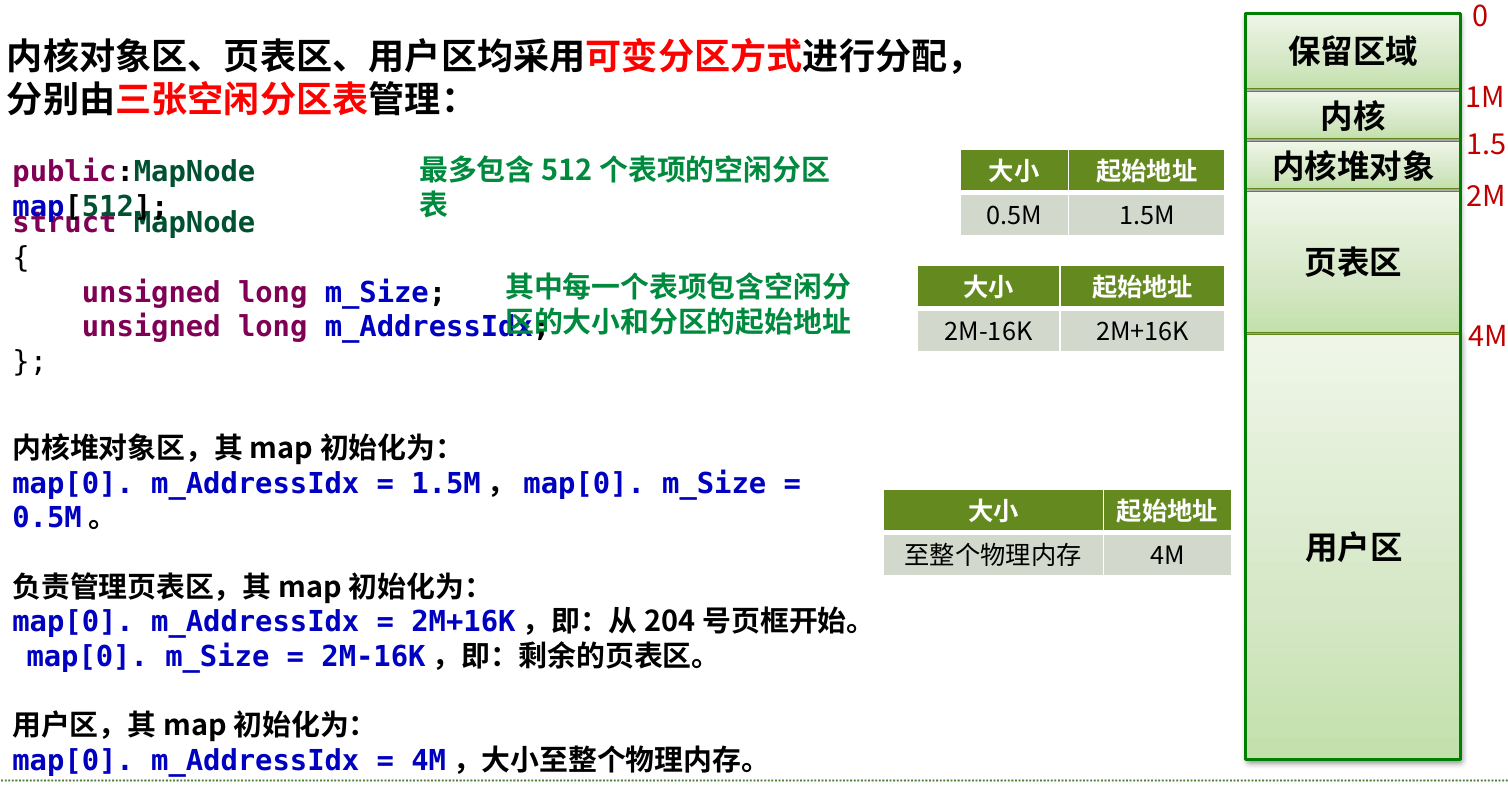
\includegraphics[width=0.85\textwidth]{figures/fig_mem_layout.png}
  \caption{UNIX V6++ 物理内存地址空间布局（图源：课程设计 PPT slide 21）}
  \label{fig:mem-layout}
\end{figure}

在\textbf{分配方式}上，原系统采用连续可变分区管理，由一张最多 512 个表项的
空闲分区表 \texttt{MapNode map[512]} 记录各空闲分区的大小与起始地址，分配算法
\texttt{Allocator::Alloc/Free}（对应 UNIX V6 中的 \texttt{malloc/mfree}）实现
首次适配与相邻分区合并。内核堆对象区、页表区、用户区分别由各自的分区表管理。

在\textbf{进程图像}上，原系统为每个进程维护一段连续的物理内存用于存放其用户态
图像，进程控制块 \texttt{Proc} 中的 \texttt{p\_addr} 字段指向该连续区域的起始
地址。其结果是：\texttt{fork} 创建子进程时需要把父进程的整段图像复制一遍；
\texttt{exec} 加载新程序时需要为其分配一段足够大的连续内存；当物理内存不足以
容纳所有进程图像时，则由 \texttt{SwapperManager} 通过盘交换区把部分进程图像
换出到磁盘，待需要时再换入。换言之，原系统的内存管理是建立在"进程图像连续且
可换出"这一前提之上的。

\section{课设任务与目标}
本次课程设计的总体任务是：在教师已实现部分离散化工作的 UNIX V6++ 代码基础上，
将内存管理方式彻底改造为离散化管理，且\textbf{不使用盘交换区}。具体可拆解为
如下三大块（对应课设 PPT 与 \texttt{readme.txt} 的要求）：

\begin{enumerate}[label=（\arabic*）]
  \item \textbf{页表系统改造}。修改 UNIX V6++ 的页表系统，使每个进程拥有独立的
        页目录（Page Directory），进程创建时动态分配页目录并写入 \texttt{CR3}
        寄存器；每个进程保留一张私有的用户页表，核心页表与 0\# 用户页表则全局共享。
  \item \textbf{内存分配方式改为位示图}。用位示图（bitmap）替代原有的连续空闲
        分区表来管理物理页框，每个 bit 对应一个 4KB 物理页框，分配与释放通过
        位运算完成。
  \item \textbf{离散化存储}。在新的页表与分配机制之上，实现四点：所有逻辑页离散
        存放；fork 采用写时复制（COW）；\texttt{exec} 为用户栈分配物理页框并直接
        挂用户页表以接纳命令行参数，省去内存复制；正文段（text）共享，在
        \texttt{Text} 结构中开数组存放分配给正文段的物理页框号。
\end{enumerate}

此外，课设明确了两条约束：其一，不使用盘交换区，且不考虑用户区内存分配不成功的
情况（即上层路径可假设分配总能成功）；其二，用户态连续地址空间的抽象应当保留——
对用户程序而言，代码段、数据段、堆、栈仍按熟悉的方式组织，不必感知物理页框是否
连续。

\section{总体设计思路}
围绕上述任务，本设计将整个改造工作划分为三个相互关联的层次，分别对应内存管理
的三个核心问题：

\begin{itemize}
  \item \textbf{页表层（虚\,$\to$\,物映射）}：解决"一个虚地址如何映射到物理地址"。
        改造的核心是让每个进程拥有独立的页目录，进程切换时通过更换 \texttt{CR3}
        而非重写页表项来完成地址空间的切换。
  \item \textbf{页框分配层（物理内存管理）}：解决"一个物理页框是否空闲、如何分配
        与回收"。改造的核心是用位示图替代连续分区表，并引入页引用计数以支撑共享
        页的生命周期管理。
  \item \textbf{进程生命周期层（fork / exec / exit）}：解决"在进程创建、图像改换、
        进程退出等关键时刻，页表与页框如何协同变化"。改造的核心是 fork 的写时
        复制、exec 的挂页表与参数栈构造、text 段的引用计数共享。
\end{itemize}

这三层并非彼此独立：页表改造决定了私有页目录与私有用户页表的存在，进而要求页框
分配器能够为它们分配离散的物理页；位示图与引用计数则是 fork 写时复制、text 段
共享得以成立的物理基础。报告的后续章节即按照"页表系统改造 $\to$ 物理页框分配
改造 $\to$ 离散化进程映像管理"的顺序展开，并在每一层中说明其与上下层的耦合关系。

\section{本地工程环境与验证目标}
作为一个底层系统项目，"能构建、能启动、能验证"本身就是实现质量的重要部分。
为此，本设计在完成算法层面改造的同时，也对本地工程环境进行了适配，使改造后的
内核能够在本地真正运行起来。

构建方面，UNIX V6++ 原生面向 Windows + MinGW 工具链，使用 NASM 汇编引导与
第二阶段加载代码，用 g++ 以 freestanding 方式编译内核 C++ 源码，再由 ld 按
\texttt{Link.ld}（输出格式 \texttt{pei-i386}，入口 \texttt{greatstart}，
\texttt{.text} 段定位于 \texttt{0xc0100000}）链接成 \texttt{kernel.exe}，最后
经 \texttt{objcopy} 转为裸二进制 \texttt{kernel.bin}。用户态程序则由 gcc 配合
用户库 \texttt{Lib\_V6++.a} 编译为 PE 可执行，由内核内的 \texttt{PEParser}
加载。运行方面，可使用 Bochs 或 QEMU（\texttt{qemu-system-i386}）加载生成的
磁盘镜像进行验证，工程 Makefile 中已提供 \texttt{make qemu} 与 \texttt{qemug}
（带 \texttt{-s -S} 供 gdb 调试）目标。

本设计的验证目标依次为：内核能够完整构建；能够由 bootloader 引导启动并进入
shell；能够在 shell 中运行用户程序（如 \texttt{ls}、\texttt{cat}、\texttt{fork}
等），并借此验证页表切换、位示图分配、写时复制与正文段共享等关键机制确实按
预期工作。工程适配的具体细节集中在第六章，对应的验证过程与结果则见第八章。
